\documentclass[11pt,a4paper,twoside]{report}
\usepackage[utf8]{inputenc}
\setlength{\parskip}{0.3cm}
\usepackage[portuguese]{babel}
\usepackage[T1]{fontenc}
\usepackage{fancyhdr}
\usepackage{amsmath}
\usepackage{amsfonts}
\usepackage{amssymb}
\usepackage{makeidx}
\usepackage{graphicx}
\usepackage{lmodern}
\usepackage{wrapfig}
%\usepackage{color}
\usepackage{color,colortbl,multirow}
\usepackage{multirow}
\usepackage[table]{xcolor}
\definecolor{lightgray}{gray}{0.9}
\usepackage{float}
%\usepackage{fourier}
\usepackage[left=2cm,right=1.5cm,top=2cm,bottom=2cm]{geometry}
\author{Bartolomeu J. Ubisse}
\pagestyle{fancy}
\renewcommand{\headrulewidth}{0pt}
\renewcommand{\footrulewidth}{1pt}
\fancyfoot[L]{ | UEM - 2017}
\fancyfoot[c]{}
\fancyfoot[r]{\thepage}
\begin{document}


\begin{figure}[htb]

\centering

\includegraphics[scale=1]{UEM-logotipo}
\end{figure}
\centering
{ \Large Universidade Eduardo Mondlane}\\[0.3cm] 
\large Faculdade de Ci\^encias\\[0.2cm]
 \large Departamento de F\'isica\\[0.5cm]

%\textsc{Electr\^onica B\'asica} \\[1cm]
\begin{flushleft}
\tt Teste 2 - E. Anal\'ogica\hspace{0.25cm} |Data:$31/05/2017$\hspace{0.25cm}|Hora:$10:00-12:00$ hrs.\\
\hrulefill
 \begin{table}[htb]
\centering
\begin{tabular}{p{16.55cm}}
\hline
\cellcolor[gray]{0.95}
Responda atentamente as perguntas que lhe s\~ao colocadas e mostre todos os passos necess\'arios.\\

 \hline
\end{tabular}
\end{table}
\end{flushleft}

\begin{enumerate}
\item Explique em que difere um trans\'istor bipolar de jun\c c\~ao (TBJ) de um trans\'istor de efeito de campo (FET).[\textit{$3.5$ Valores}]
\item Explique como \'e que surge o canal num NMOS de tipo enriquecimento.[\textit{$3.5$ Valores}]
\item Explique o que entende por corrente de engate num SCR.[$3.0$ Valores]
\item Detemine o ganho de tens\~ao do amplificador da fig.\ref{f2} considerando que $V_T=26$mV.[\textit{$6.0$ Valores}]
\item Determine as magnitudes dos resistores do circu\'ito da fig.\ref{a2} considerando que $V_p=-3$V, $I_{DSS}=9$mA, $V_G=5$V,$I_D=4$mA e $V_D=11$V.[\textit{$4.0$ Valores}]
\end{enumerate}
  \noindent
\begin{minipage}[c]{5cm}
 \begin{figure}[H]
\centering
\includegraphics[scale=0.7]{test2tbj}
\caption{}
\label{f2}
\end{figure}
\end{minipage}\hfill
\begin{minipage}[c]{9cm}
\begin{figure}[H]
\centering
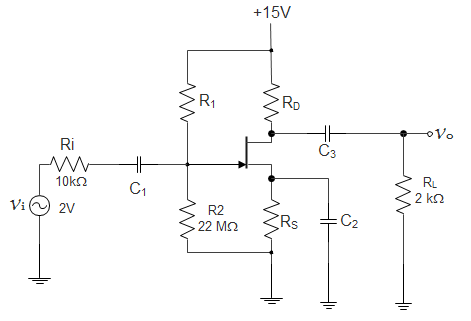
\includegraphics[scale=0.7]{JFET1}
\caption{}
\label{a2}
\end{figure}
\end{minipage}



\vspace{1.5cm}

\huge{Bom Trabalho !}

\newpage
\normalsize
 Teste 2 - E. Anal\'ogica\hspace{0.25cm} |Data:$31/05/2017$\hspace{0.25cm}|Hora:$10:00-12:00$ hrs |Corre\c c\~ao.\\
\hrulefill
\begin{enumerate}
\item Os FETs s\~ao unipolares enquanto que os TBJs s\~ao bipolares; Os FETs usam campo el\'ectrico para controlar a condutibilidade do seu canal enquanto que os TBJs usam a corrente de base; Os FETs comparativamente com os TBJs tem uma alta imped\^ancia de entrada, tem uma comuta\c c\~ao r\'apida, dimens\~oes pequenas, maior estabilidade t\'ermica, menor ru\'ido, etc. 
\item Num NMOS de tipo enriquecimento o canal surge quando se aplica uma diferen\c ca de potencial entre a porta e a fonte com um valor superior que a tens\~ao limiar, isto \'e, $V_{GS}>V_t$. Durante a aplica\c c\~ao deste $V_{GS}$, as lacunas da parte superior do substrato junto \'a camada do diel\'ectrico s\~ao repelidas para a parte mais inferior do substrato e, nessa desloca\c c\~ao v\~ao deixando i\~oes negativos referentes \`as impurezas aceitadoras. Ainda mais, o potencial positivo na porta atrai mais electr\~oes junto da regi\~ao da carga espacial resultante de saida das lacunas. \`A medida que se vai aumentando o valor de $V_{GS}$, mais ser\'a a concentra\c c\~ao de elect\~oes pr\'oximo \'a superf\'icie do substrato e logo que $V_{GS}\geq V_t$ uma região $n$ ser\'a criada  conectando-se deste modo  as  regiões  de  fonte  e  dreno e, com aplica\c c\~ao de $V_{DS}$ uma corrente circular\'a entre a fonte e o dreno. 
\item Corrente de engate (latching current) \'e a m\'inima corrente an\'odica necess\'aria para que mesmo com a retirada do pulso na porta do tir\'istor ele continue no estado ativado.  
\item Determina\c c\~ao de ganho de tens\~ao\\
\noindent
i) An\'alise cc\\
\begin{minipage}[c]{2.5cm}
\begin{figure}[H]
\centering
\includegraphics[scale=0.8]{analisecc}
\caption{}
\label{f4}
\end{figure}
\end{minipage}\hfill
\begin{minipage}[c]{11cm}
{$R_{BB}=\frac{R_1\times R_2}{R_1+R_2}\Longrightarrow R_{BB}=\frac{39000\times 3900}{39000+3900}=3545.45\Omega$\\

$V_{BB}=\frac{R_2}{R_1+R_2}\times V_{CC}\Longrightarrow V_{BB}=\frac{3900}{39000+3900}\times 19 = 1.73 V$\\

$R=R_3+R_4=330+1100=1430\Omega$\\

$I_C=\beta I_B$\\
$I_B+I_C=I_E \Longrightarrow I_E=(\beta +1)I_B$\\

$V_{BB}=I_BR_{BB}+V_{BE}+I_ER_E\Longrightarrow V_{BB}=I_B\left( R_{BB}+(1+\beta)R\right)+ V_{BE}$\\

Assim: $I_B=\frac{V_{BB}-V_{BE}}{R_{BB}+(1+\beta)R}\Longrightarrow I_B=\frac{1.73-0.7}{3545.45+(1+100)1430}=6.94\mu A$\\

$I_C=\beta I_B\Longrightarrow I_C=100\times 6.94\mu A =0.69 mA$\\

$I_E=(\beta +1)I_B \Longrightarrow I_E=(100 +1)\times6.94\mu A= 0.70mA$
}
\end{minipage}

\hrulefill

ii) An\'alise ac

\noindent
\begin{minipage}[c]{5cm}
\begin{figure}[H]
\centering
\includegraphics[scale=0.65]{analiseac}
\caption{}
\label{f4}
\end{figure}
\end{minipage}\hfill
\begin{minipage}[c]{8cm}
{$r_{\pi}=\frac{V_T}{I_B}\Longrightarrow r_{\pi}=\frac{26mV}{6.94\mu A}=3745.22\Omega
 $\\

$i_b=\frac{v_i}{r_{\pi}+(1+\beta)R_3}$\\

$i_c=\beta \times i_b\Longrightarrow i_c=\frac{\beta v_i}{r_{\pi}+(1+\beta)R_3}$\\

$v_o=i_c\times R_C\Longrightarrow v_o=\frac{\beta R_C }{r_{\pi}+(1+\beta)R_3}\times v_i$\\

$A_v=\frac{v_o}{v_i}\Longrightarrow A_v=\frac{\beta R_C }{r_{\pi}+(1+\beta)R_3}$\\

$ A_v=\frac{100\times4700\Omega}{3745.22\Omega+(1+100)\times 330\Omega}=12.67$\\
}
\end{minipage}

\item Determine as magnitudes dos resistores do circu\'ito da fig.\ref{a2} considerando que $V_p=-3$V, $I_{DSS}=9$mA, $V_G=5$V,$I_D=4$mA e $V_D=11$V.\\

{$V_{DD}=R_DI_D+V_D\Longrightarrow R_D=\frac{V_{DD}-V_D}{I_D}\Longrightarrow R_D=\frac{(15-11)V}{4mA}=1k\Omega$\\

$I_D=I_{DSS}\left( 1-\frac{V_{GS}}{V_{GS (off)}}\right) ^2\Longrightarrow 4mA=9mA\left( 1+\frac{V_{GS}}{3}\right) ^2\Longrightarrow V_{GS}=-5V$ ou $ V_{GS}=-1V$; \\

 \textit{Solu\c c\~ao}:$V_{GS}=-1V$\\

$V_{GS}=V_G-V_S\Longrightarrow V_S= (5+1)V= 6V$;  $V_{DS}=V_D-V_S=(11-6)V=5V$\\

$V_{DD}=I_DR_D+V_{DS}+I_DR_S\Longrightarrow R_S=\frac{V_{DD}-V_{DS}-I_DR_D}{I_D}\Longrightarrow R_S=\frac{15V-5V-4.10^{-3}A\times10^3\Omega}{4\times10^{-3}A}=1.5k\Omega$\\

$I_G=0A \longrightarrow V_G=V_{GG}=5V$\\
$V_{GG}=\frac{R_2}{R_1+R_2}V_{DD}\Longrightarrow R_1=\left( \frac{V_{DD}}{V_{GG}}-1\right)R_2 \Longrightarrow R_1=\left( \frac{15}{5}-1\right) \times 22\times 10^6 \Omega=44M\Omega $
}


\end{enumerate}

\end{document}